\documentclass[a4paper, 10pt]{article}
\usepackage[utf8]{inputenc}
\usepackage[spanish] {babel}
\usepackage{amsfonts}
\usepackage{amssymb}
\title{Trabajo Practico 3}
\usepackage{tpalgo3}
\usepackage{caratula}
\usepackage{amssymb}
\usepackage[pdftex]{graphicx}
\usepackage{hyperref}


\setlength{\leftmargin}{10cm}
\setlength{\rightmargin}{10cm}
\setlength{\oddsidemargin}{-1cm}
\setlength{\evensidemargin}{-1cm}
\setlength{\topmargin}{-1cm}
\setlength{\textwidth}{18cm}
\setlength{\textheight}{25cm}

\usepackage{fancyhdr}
\pagestyle{fancy}
\fancyhf{}
\fancyhead [L]{\scriptsize Trabajo Práctico N$^{\circ}$2}
\fancyhead [R]{\scriptsize Aronson, Ravasi}%1{20pt}
\fancyfoot[C]{\thepage}
\renewcommand{\footrulewidth}{0.4pt}

\begin{document}
\materia{Algoritmos y Estructuras de Datos III}
\submateria{Segundo Cuatrimestre de 2010}
\titulo{Trabajo Practico N$^{\circ}$3}
\grupo{Grupo 14}
\integrante{Aronson Alex}{443/08}{alexaronson@gmail.com}
% \integrante{Nahabedian Leandro Ezequiel}{250/08}{leanahabedian@hotmail.com}
\integrante{Ravasi Nicolás}{53/08}{nravasi@gmail.com}
\maketitle
\newpage

\tableofcontents
\newpage

\section{Archivos incluidos en este TP}
Además de todos los archivos provistos por la cátedra, incluimos varios jugadores hechos por nosotros, como ser

\begin{itemize}
\item $minimax.cpp$: Jugador minimax, sin poda
\item $src/alfabeta.cpp$: Jugador minimax, con poda alfabeta
\item $src/timer\_minimax.cpp$: Jugador minimax, sin poda, con contador de cantidad de jugadas vistas
\item $src/timer\_alfabeta.cpp$: Jugador minimax, con poda alfabeta, con contador de cantidad de jugadas vistas
\item $src/scorer1.cpp$: Primera heurística, recibe 2 parámetros (valor adyacente y valor exponente)
\item $src/scorer2.cpp$: Segunda heurística, recibe 2 parámetros (valor adyacente y valor exponente)
\item $src/scorer3.cpp$: Tercera heurística, recibe 2 parámetros (valor adyacente y valor exponente)
\item $src/scorer4.cpp$: Cuarta heurística, recibe 3 parámetros (valor ficha, adyacente y exponente)
\item $src/jfin1.cpp$: Primer jugador mixto heurístico/minimax, recibe 3 parámetros (profundidad a mirar, adyacente y exponente)
\item $src/jfin2.cpp$: Segundo jugador mixto heurístico/minimax, recibe 4 parámetros (profundidad a mirar, offset, adyacente y exponente)
\item $src/jfin3.cpp$: Tercer jugador mixto heurístico/minimax, recibe 3 parámetros (profundidad a mirar, adyacente y exponente)
\item $src/jfin4.cpp$: Cuarto jugador mixto heurístico/minimax, recibe 4 parámetros (profundidad a mirar, valor ficha, adyacente y exponente)
\item $src/jfin5.cpp$: Quinto jugador mixto heurístico/minimax, recibe 6 parámetros (jugadas iniciales para no hacer minimax, profundidad a mirar hasta medio juego, profundidad a ver luego, valor ficha, adyacente y exponente)
\item $Makefile$ provisto por la cátedra pero modificado para que compile nuestros sources
\item Múltiples scripts que usamos para testear los jugadores, por ejemplo $minimax\_rojo$ y $alfabeta\_verde$ para testear los timer; $sc4\_final\_rojo$, $jf4\_final\_rojo$ y $jf5\_final\_rojo$ para probar los jugadores contra todos los otros; $sc4\_rojo$, $sc4\_verde$ y $sc3\_rojo$ para testear múltiples parámetros de una pasada

\end{itemize}

\newpage

\section{Primera Parte}
\subsection{Minimax}
\subsubsection{Presentación del algoritmo}

Lo primero que hicimos para encarar este problema fue un algoritmo Minimax, que se encargara de ver todas las posibilidades para cada instancia del tablero, una vez que se vieran todas éstas, para cada una se ven todas las jugadas posibles del rival, para éstas se ven las siguientes del primer jugador, y así hasta llegar a una situación en la cual no se puede efectuar movida alguna. En ese caso, se llama a una función que determina el puntaje del tablero. Si pensamos que estamos por hacer la última jugada, haciendo el minimax tenemos el resultado que daría hacer cada una de las movidas posibles, dada la naturaleza del juego, siempre eligiríamos aquella que nos permita obtener el mayor puntaje posible. Por lo tanto dadas todas esas movidas, sólo elegiremos una, en cuyo caso podemos asignar a nuestra situación previa a esa movida el puntaje de la movida que elegiríamos. Si pensamos hacia atrás, el rival tendría todos estos puntajes correspondientes a cada una de nuestras movidas, y trataría de elegir la que es mejor para él, dada la condición de suma-cero del juego, esto sería la que es peor para nosotros. Por lo tanto podemos saber cual elegiría él, y así asignar un puntaje a la movida previa del mínimo de los scores, y así hacia arriba hasta llegar a la primera movida, eligiendo siempre el máximo para nuestras jugadas (que representan la mejor opción) y el mínimo para las de rival (que representan la mejor opción de él).

Dicho esto, nuestro algoritmo hace exactamente esto, desarrolla todo el árbol de posibilidades desde el principio, asigna los valores a las jugadas finales y selecciona alternadamente los mínimos y máximos según corresponda para devolver la mejor jugada posible considerando un juego óptimo por parte del rival. Por lo tanto, presentamos el pseudocódigo de nuestro algoritmo minimax.\\

\nuevoAlgo{Algoritmo 1}{minimax() $\rightarrow$ $res$ : $Nat$.
Devuelve el valor de la mejor jugada para un jugador dada la posición.} \\
\\
\begin{tabular}{rp{17cm}}
1: & minimax ()\ \{\vspace{0,1cm} \\
2: & \hspace{0,5cm}   int $maximo$ : VALOR\_MINIMO \vspace{0,1cm} \\
3: & \hspace{0,5cm}   vector$<$jugada$>$ jugadasposibles: calcularJugadasPosibles()\vspace{0,1cm} \\
4: & \hspace{0,5cm}   $\iif$ vacio(jugadasposibles) \{\vspace{0,1cm} \\
5: & \hspace{1cm}     devolver $scoretablero$ \vspace{0,1cm} \\
4: & \hspace{0,5cm}   $\forall i \in$  [0, jugadasposibles.tam)\{\vspace{0,1cm} \\
5: & \hspace{1cm}            aplicarEnTablero($i$) \{\vspace{0,1cm} \\
6: & \hspace{1cm}            int $score$: $-$minimax()\vspace{0,1cm} \\
7: & \hspace{1cm}            $maximo$ $=$ max($score$,$maximo$)\vspace{0,1cm} \\
8: & \hspace{1cm}            quitarEnTablero($i$)\vspace{0,1cm} \\
9: & \hspace{1cm}         \}\vspace{0,1cm} \\
10: & \hspace{0.5cm}         devolver maximo \vspace{0,1cm} \\
11: & \}\\ \vspace{0,1cm} \\
\end{tabular}


\subsubsection{Complejidad del algoritmo}
Primero se calculan la cantidad de jugadas posibles, esto lo hacemos recorriendo casilla por casilla fijándonos si se puede poner una ficha, primero recorremos horizontalmente y luego verticalmente, si se puede, se agrega al final de un vector en tiempo constante. Por lo tanto, ver las jugadas posibles es $O(n^{2})$, siendo $n$ la cantidad de filas (o columnas) del tablero.
Si el tamaño resultante de este vector es 0, se llama al puntuador de tablero que devuelve el score del mismo, esta función es una adaptación de la que usa el juez para calcular el puntaje del tablero y tiene complejidad $O(n^{2})$. En caso contrario, vamos a recorrer todas las jugadas posibles. Si lo analizamos, para toda posición del tablero, esa posición puede ser usada por una ficha como primer casilla de dos maneras (en vertical u horizontal), excepto la última fila y la última donde sólo se puede poner de una manera. Esto nos da $2(n^{2}-n)$ jugadas posibles en peor caso, o sea, del orden de $n^{2}$. Para cada una de estas se va a aplicar la recursión para ir formando el árbol. Ésta se va a aplicar $n^{2}/2$ veces seguidas, porque si se tiene el tablero de $n x n$, la cantidad de casillas es $n^{2}$, si tenemos que cada jugada ocupa 2 casillas, al terminar un partido se van a haber hecho a lo sumo $n^{2}/2$ jugadas. Por lo tanto, tenemos una función que cuesta, sin contar la recursión, $O(n^{2})$, y un "árbol $n^{2}$-ario", con cada nodo teniendo $n^{2}$ hijos, por lo tanto, la cantidad de nodos total es, aplicando la propiedad de árboles completos, del orden de cantidad de hijos$^{altura + 1}$, esto es, $(n^{2})^{(n^{2} +1)}$, o sea, $n^{(2n^{2}+2)}$. Por lo tanto, multiplicando por la complejidad de cada ejecución, podemos decir que la complejidad total es $O(n^{2} * n^{(2n^{2}+2)})$ = $O(n^{2n^{2}+3})$ 
.

\subsection{Poda alfa-beta}

Como se puede ver, el algoritmo minimax tiene complejidad exponencial, y no sólo eso, sino que además está garantizado de recorrer todos y cada uno de los nodos del árbol, aún cuando esté recorriendo ramas del árbol que no tengan posibilidad de ser usadas porque éstas incluyen jugadas muy malas para uno u otro, y dada la naturaleza del algoritmo de elegir siempre la mejor jugada para cada situación, es obvio que estas no van a ser parte de la solución. Por lo tanto, podemos implementar una poda alfa-beta, que, como toda poda, no va a reducir la complejidad total del algoritmo, ya que en peor caso se va seguir recorriendo todo el árbol, pero en caso promedio se van a podar muchos nodos y el tiempo de ejecución va a ser menor.

Para esto, usamos básicamente el mismo código, pero agregando una condición que interrumpiera la recorrida de las jugadas posibles para en caso de obtener un resultado parcial que haga que no sirva seguir calculando el resto de las jugadas para esa posición. Así, utilizamos dos parámetros, alfa y beta. En estos parámetros que tiene como valor inicial los valores infinitamente pequeños y grandes
respectivamente almacenaremos los valores máximos y mínimos correspondientes a la mejor eleccion del camino elegido. En la variable alfa almacenaremos constantemente la eleccion del valor mas alto y en la variable beta la elección del mas bajo. Este algoritmo desarrollara la poda cuando el valor que se este recorriendo en ese momento sea peor que el valor de alfa o beta para los caminos maximos y minimos respectivamente\\

\nuevoAlgo{Algoritmo 2}{alfabeta($alfa$ : $Nat$, $beta$ : $Nat$) $\rightarrow$ $res$ : $Nat$.
Devuelve el valor de la mejor opción a lo largo del camino MAX, esto implicará por lo tanto la elección del valor más alto} \\
\\
\begin{tabular}{rp{17cm}}
 	1: & alfabeta ()\ \{\vspace{0,1cm} \\
 	2: & \hspace{0,5cm} int $maximo$ : VALOR\_MINIMO \vspace{0,1cm} \\
 	3: & \hspace{0,5cm} vector$<$jugada$>$ jugadasposibles: calcularJugadasPosibles()\vspace{0,1cm} \\
 	4: & \hspace{0,5cm} $\iif$ vacio(jugadasposibles) \{\vspace{0,1cm} \\
 	5: & \hspace{1cm} devolver $scoretablero$ \vspace{0,1cm} \\
 	4: & \hspace{0,5cm} $\forall i \in$ [0, jugadasposibles.tam)\{\vspace{0,1cm} \\
 	5: & \hspace{1cm} aplicarEnTablero($i$) \{\vspace{0,1cm} \\
 	6: & \hspace{1cm} int $score$: $-$alfabeta($-beta$, $-alfa$)\vspace{0,1cm} \\
 	7: & \hspace{1cm} $alfa$ $=$ max($score$,$alfa$)\vspace{0,1cm} \\
 	8: & \hspace{1cm} quitarEnTablero($i$)\vspace{0,1cm} \\
	9: & \hspace{1cm} $\iif$ ($beta$ $\leq$ $alfa$)  \{\vspace{0,1cm} \\
 	10: & \hspace{1,5cm}  break \vspace{0,1cm} \\
 	11: & \hspace{1cm} \}\vspace{0,1cm} \\
 	12: & \hspace{0.5cm} devolver $alfa$ \vspace{0,1cm} \\
 	13: & \}\\ \vspace{0,1cm} \\
 	\end{tabular} 

\subsection{Comparación entre los dos algoritmos}

Puede verse que en peor caso, la poda alfa-beta tiene la misma complejidad que el minimax, ya que si no se entra en la guarda del $if$ nunca se hace break y por ende se va a terminar recorriendo todas las jugadas posibles en todos los casos. Pero, aún cuando no se reduzca la complejidad, vamos a demostrar que la poda es muy efectiva puesto que en la práctica se reduce mucho la cantidad de jugadas analizadas.

Para esto vamos a introducir dos nuevos jugadores, $timer\_minimax.cpp$ y $timer\_alfabeta.cpp$, los dos son exactamente iguales a sus predecesores pero tienen un contador el cual inicializan en 0 e incrementan por cada jugada que miran en el tablero. Al final de la ejecución, cuando se ejecuta el SIGTERM, simplemente imprimimos por pantalla este contador y tendremos la cantidad de jugadas que analizó el jugador.

Dada la inherente imposibilidad de correr los jugadores en un tablero de más de 4 filas en un tiempo razonable, y que el tablero de 3x3 es demasiado trivial, nos centramos en el estudio del comportamiento de los jugadores para un tablero de 4x4, comparando la cantidad de jugadas que analizan los jugadores tanto cuando juegan con rojo como cuando juegan con verde. Presentamos los resultados a continuación

Para rojo:

\begin{center}
\begin{tabular}{|c|c|c|}
\hline
Jugadores & \multicolumn{1}{l|}{Cant. jugadas vistas Minimax} & \multicolumn{1}{l|}{Cant. jugadas vistas Alfabeta} \\ \hline
Labi & 6.286.522 & 208.433 \\ \hline
Wabi & 6.277.647 & 207.930 \\ \hline
Fixed & 6.289.042 & 207.497 \\ \hline
Heur & 6.278.636 & 206.945 \\ \hline
Heurb & 6.266.801 & 207.071 \\ \hline
Rand & 6.266.853 & 207.894 \\ \hline
\end{tabular}
\end{center}

\vspace{0,15cm}


\begin{center}
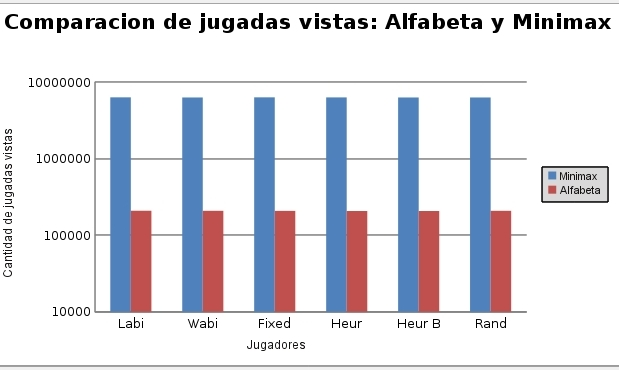
\includegraphics[scale=0.70]{graficos/1-1.jpg} \\
\scriptsize{\textsf{\textbf{Gr\'afico 1.1, comparación de las jugadas vistas entre alfabeta y minimax para un tablero de 4x4 contra los diferentes jugadores de la cátedra, jugando con rojo}}}  \\
\end{center}


\vspace{1cm}

Para verde:

\begin{center}
\begin{tabular}{|c|c|c|}
\hline
Jugadores & Cant. jugadas vistas Minimax & Cant. jugadas vistas Alfabeta \\ \hline
Labi & 231.328 & 11.089 \\ \hline
Wabi & 372.926 & 16.615 \\ \hline
Fixed & 373.880 & 16.668 \\ \hline
Heur & 170.709 & 7.925 \\ \hline
Heur B & 170.709 & 7.849 \\ \hline
Rand & 372.287 & 7.939 \\ \hline
\end{tabular}
\end{center}

\vspace{0,15cm}

\begin{center}
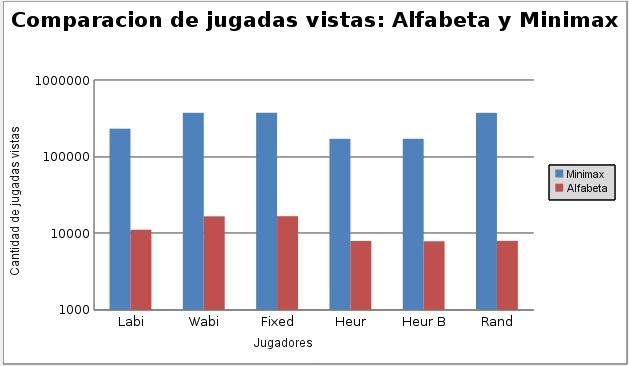
\includegraphics[scale=0.80]{graficos/1-2.jpg} \\
\scriptsize{\textsf{\textbf{Gr\'afico 1.2, comparación de las jugadas vistas entre alfabeta y minimax para un tablero de 4x4 contra los diferentes jugadores de la cátedra, jugando con verde}}}  \\
\end{center}


Puede verse que en todos los casos la cantidad de jugadas analizadas por alfabeta es muy inferior al del minimax, 3\% de las movidas para rojo y 5\% para verde; es evidente que la mejora es sustancial y dado que terminan jugando igual, no cabe otra que concluir que la poda alfabeta es siempre preferible por sobre el minimax común, de modo que la usaremos en el resto del TP siempre que mencionemos al minimax.

\newpage


\section{Segunda parte}
\subsection{Evaluación del tablero}

\subsubsection{Primera heurística}

Sabiendo la imposibilidad de aplicar el alogritmo minimax para un tablero siquiera mediano, debíamos encontrar un algoritmo que dada una posición del tablero sea capaz de hacer una evaluación de la misma para determinar qué tan buena o mala es, de manera rápida. Para esto, sabíamos que obviamente había que tener en cuenta el puntaje acumulado hasta ahora por las islas en el tablero, ya que esto es lo que básicamente determina quién gana, pero también consideramos importante la posibilidad que tiene cada jugador de expandirse, esto es, de poner nuevas fichas cerca de las que ya tiene, ya que esto permitirá expandir su isla, lo que le dará más puntos que poner una ficha totalmente aislada.

De esta manera, nuestro primer intento de evaluador tomaba la función $game\_score$ del juez, que determina el puntaje total de los jugadores dada una posición tomando en cuenta el valor de las islas; y le agregamos una función aparte que determine si para cada posición en el tablero donde hay una ficha del jugador, existe la posibilidad de adjuntar una (o más) fichas adyacentes a la misma, y si existe esa posibilidad (o sea, si la función $puedo\_poner\_adyacente$ da true, que sume 1 al puntaje de ese jugador. De esta manera, un jugador recibiría una evaluación favorable si tiene piezas conexas y además espacio para expandirse. Con esta heurística, creamos el jugador goloso $scorer1.cpp$.

\subsubsection{Segunda heurística}


Hecho esto, nos resultó evidente que no era conveniente evaluar una posición donde sólo se puede expandir para un costado de la misma manera que una posición donde se puede expandir hacia tres. Por lo tanto, modificamos la función $puedo\_poner\_adyacente$ de manera tal que devolviese un entero indicando hacia cuántos lugares puede hacerlo, en lugar de un bool; y sumar esa cantidad al total para cada casilla del tablero; con esta simple modificación obtuvimos $scorer2.cpp$.

\subsubsection{Tercera heurística}


Ahora bien, si bien la heurística era razonablemente buena, no era parametrizable en lo más mínimo, ya que lo que se sumaba al score por la cantidad de espacios adyacentes donde se pudiera poner una ficha era fijo. De esta manera, pensamos que por cada uno de estos espacios se podía sumar no solamente 1, sino un parámetro especificado por el usuario, y no sólo esto, sino que podíamos hacer que dada una cantidad de espacios libres, estos fueran elevados a una potencia para así poder alternar entre qué es lo que tuviera más prioridad, el puntaje de las islas o el de los espacios libres adyacentes. Con esta heurística, obtuvimos nuestro primer jugador parametrizable, el jugador goloso $scorer3.cpp$

\subsubsection{Cuarta heurística}


Con la tercera heurística obtuvimos buenos resultados, pero aún así sabíamos que no era lo ideal puesto que dada la forma de calcular las adyacencias había casillas que podían estar siendo contadas como adyacencias varias veces (por ejemplo, con fichas dispuestas en forma de U, la casilla central sería contada tres veces, una por cada una de las posiciones que la rodean que tienen una ficha). Además, queríamos modificar la heurística de manera tal que el puntaje de adyacencias no fuera contado separado del de las islas sino al mismo tiempo, porque de esta manera contaría las adyacencias casi como piezas, ya que si uno tiene muchas adyacencias el oponente no puede hacer nada para evitar que el jugador se expanda por las mismas. Pero esto implicaba desechar completamente la función $game\_score$ ya que esta no nos permitía hacer esto de la manera que se nos había ocurrido, por lo tanto ideamos una función nueva que calculara el puntaje del tablero a nuestra manera, y que a la misma le pudiéramos si quisiéramos sumar para cada posición los adyacentes libres. Así, tenemos una matriz aparte de la que contiene las fichas, la matriz $marc$ que iniciamos toda en 0 y nos va a indicar qué posiciones ya fueron vistas, recorremos una a una las posiciones, de encontrar una ficha de un color, marcamos esa posición en $marc$ y hacemos BFS sobre esa posición, recorriendo hacia todos los costados y marcando tanto las fichas del mismo color como las posiciones donde se pueden poner fichas adyacentes. De esta manera podemos parametrizar el valor que tiene tanto una ficha como una posicion libre adyacente; y elevar a la potencia pasada por parámetro directamente la suma de éstas dos cosas juntas. Con esta nueva heurística hicimos el jugador goloso $scorer4.cpp$.

\subsection{Demostración de la complejidad}

Vamos a demostrar solamente la complejidad de la heurística final, puede verse que las demás heurísticas no tienen complejidad mayor. En la función, lo primero que hacemos es setear todos los valores en la matriz $marc$ en 0, esto tiene complejidad $O(n^{2})$ con $n$ la cantidad de filas del tablero. Luego, recorremos todas las casillas nuevamente, preguntando si están marcadas o no. En caso de que lo estén, las salteamos, en caso de que no y que además no estén vacías, las marcamos y además recorremos toda la isla; moviéndonos hacia los cuatro costados y en caso de encontrar una ficha del mismo color no marcada, agregándola a la cola. De esta manera hacemos un BFS que nos asegura que todas las posiciones de la cola van a ser recorridas. Puede verse que para una posición, mirar sus cuatro adyacentes y determinar en las que están libres si puede colocarse una ficha toma tiempo constante. También puede verse que si una casilla está marcada, no se va a cumplir la condición del $if$ y por lo tanto no se va a tener en cuenta. El BFS no tiene una complejidad dada, es lineal sobre el tamaño de la isla, ésta puede ser como mucho $n^{2}$ pero esto implicaría marcar todas las casillas durante una sola pasada. Por ende, como mucho accedemos a cada posición dos veces, una para marcarla y otra recorriéndola en el doble for original pero no teniéndola en cuenta puesto que ya está marcada. Por lo tanto, la complejidad total es $O(n^{2})$

\subsection{Jugadores golosos}
\subsubsection{Compejidad}

Con cada una de las heurísticas desarrollamos un jugador goloso, cuyo funcionamiento es siempre el mismo (lo que varía es la heurística): dado su turno de mover, crea una lista con todas las jugadas posibles, para cada una aplica esa movida y calcula el puntaje del tablero según la heurística que tiene asociada, de todos esos toma el máximo valor y lo devuelve como jugada. Dado que la implementación de este jugador, en todas sus versiones, es muy básica, es importante desarrollar una buena heurística para que éste juegue bien. 

Dicho esto, tenemos las heurísticas que sabemos que tienen complejidad $O(n^{2})$, siendo $n$ la cantidad de filas del tablero; ya habíamos dicho que dada una posición, en peor caso hay $n^{2}$ jugadas posibles para hacer, como para cada una se aplica la heurística, para hacer una jugada el algoritmo cuesta $O(n^{4})$. Sabiendo que la cantidad de jugadas que se van a hacer en una partida está acotada por $n^{2}/2$, las jugadas propias están acotadas por $n^{2}/4$. Por lo tanto, la complejidad total para una partida es  $O(n^{6})$

\subsubsection{Elección de parámetros}

Para elegir los mejores parámetros para $scorer4$, teníamos tres diferentes variables para cambiar, el valor de la ficha, el valor de una casilla adyacente a la isla donde se podría en el futuro poner una ficha y el exponente al cual se eleva el valor de isla + adyacentes. Ya de entrada vimos que había valores de exponentes que debíamos descartar de plano, puesto que exponentes mayores que 3 daban malos resultados contra los jugadores de la cátedra (por ejemplo, perdiendo todos los partidos jugados contra $heurb$). Por lo tanto, nos centramos en los que consideramos válidos.

Con esto, para verificar los mejores, decidimos simplemente hacer jugar al jugador contra sí mismo pero con otros parámetros, primero descartamos los inviables y después hicimos un mini-torneo.

Con esto, vimos que el exponente de valor uno tampoco era útil ya que perdía contra los mismos parámetros pero con exponente 2. De la misma manera, cualquier jugador con valor adyacente 1 le gana a cualquier otro con valor mayor, de manera tal que el valor ideal para el segundo parámetro siempre es 1.

Así, limitando el máximo a 5 por conveniencia, nos quedamos con 10 combinaciones de parámetros que hicimos competir para obtener la mejor. Lanzando al scorer con 4 de valor de ficha, 1 de adyacente y 2 de exponente, nos encontramos con que les ganaba a todos jugando con rojo, y les ganaba a varios incluso con verde. Así con esta sola pasada, nos quedamos con (1,1,2; 2,1,2; 3,1,2 y 5,1,2), que eran con los que perdía jugando con verdes. Esto significa, el mejor parámetro para el exponente es 2.

Dicho esto, lanzamos a todos los jugadores a jugar contra los otros con verde, de manera tal de encontrar cual es el ''menos malo'', o sea, el que pierde por menos considerando la ventaja que jugar con rojo implica. De esta manera, corrimos cada uno de los jugadores contra los otros cuatro y anotamos su margen de derrota (por lo tanto, un valor mayor significa que ese jugador es peor). Presentamos a continuación la tabla y el gráfico de los resultados obtenidos.

\begin{center}

\begin{tabular}{|c|c|c|c|c|c|c|}

\hline
 & \multicolumn{1}{l|}{Valor Ficha 1} & \multicolumn{1}{l|}{Valor Ficha 2} & \multicolumn{1}{l|}{Valor Ficha 3} & \multicolumn{1}{l|}{Valor Ficha 4} & \multicolumn{1}{l|}{Valor Ficha 5} & \multicolumn{1}{l|}{Promedio} \\ \hline
Valor Ficha 1 & -1000 & 34814 & 34814 & 35721 & 35721 & 35267.5 \\ \hline
Valor Ficha 2 & 10954 & -1000 & 14000 & 19287 & 26230 & 17617.75 \\ \hline
Valor Ficha 3 & 7746 & 7746 & -1000 & 19287 & 23065 & 14461 \\ \hline
Valor Ficha 4 & 6928 & 6928 & 14000 & -1000 & 19799 & 11913.75 \\ \hline
Valor Ficha 5 & 14283 & 14283 & 0 & 13856 & -1000 & 10605.5 \\ \hline

\end{tabular}

\end{center}

\begin{center}

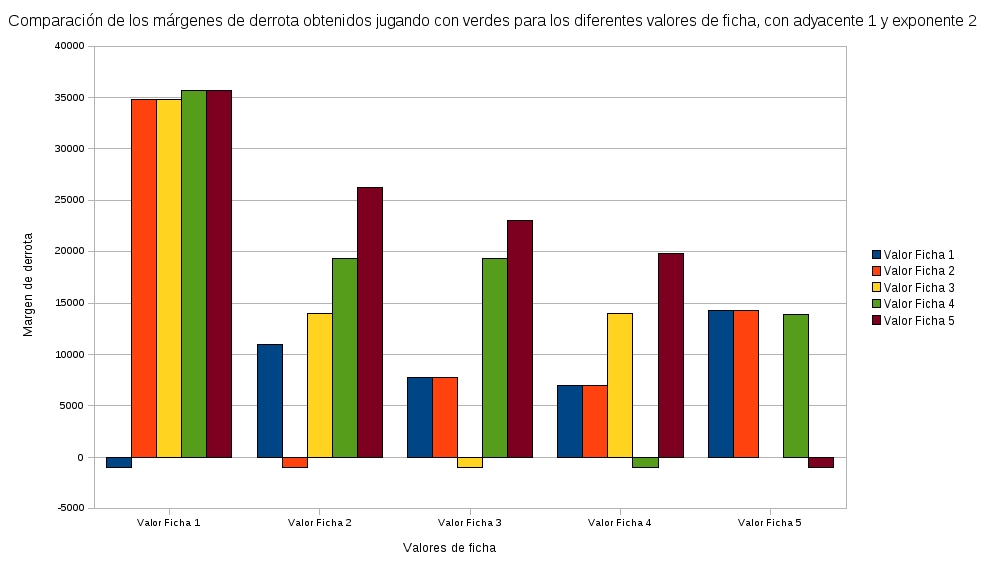
\includegraphics[scale=0.50]{graficos/2-3.jpg} \\
\scriptsize{\textsf{\textbf{Gr\'afico 2.1, comparación de los márgenes de derrota (x1000) obtenidos jugando con verdes para los diferentes valores de ficha, con adyacente 1 y exponente 2}}}  \\
\end{center}

Asignamos un valor de -1000 para los jugadores contra los mismos parámetros puesto que el análisis no reviste utilidad. 

Dado el promedio obtenido en la tabla, podemos observar que un valor de ficha de 5, un valor de adyacente de 1 y un exponente de 2 es el mejor parámetro ya que sus márgenes de derrota contra los otros jugando con verde son los menores (incluso, es el único que no pierde contra otro jugador de esos con verdes), los demás pierden por más puntos. Para asegurarnos que no fuera que el jugador fuera mejor cuanto más incrementásemos el valor de la ficha, probamos correrlo contra los mismos parámetros pero con 6 de ficha; obtuvimos que con rojo ganaba por 20.688 y con verde perdía por 19.799, por lo tanto dado que su margen de victoria es mayor que el de derrota, es 5,1,2 es el mejor parámetro.

\newpage

\section{Tercera Parte}
\subsection{Jugadores finales}
\subsubsection{Primer jugador}

Si bien los jugadores golosos juegan de una manera más o menos razonable, su limitación es evidente puesto que si bien pueden discernir una jugada muy mala de una muy buena, no tiene posibilidad de ver más allá de la heurística. Ya vimos que el algoritmo minimax (o su mejora la poda alfa-beta) es inaplicable para tableros se podría decir "no triviales", aún cuando su juego es perfecto. Por lo tanto, es necesario encontrar un equilibrio, un algoritmo que tenga la capacidad de ver jugadas a futuro pero que a su vez use una heurística sacrificando exactitud para ganar en tiempo.
Con esta idea, decidimos programar los jugadores finales, copiando el código de la poda alfa-beta (puesto que ya demostramos que ésta es mejor que el minimax así solo) pero limitando la cantidad de niveles a hacer minimax (esta cantidad va a ser parámetro), y haciendo que una vez agotados los niveles se llame no al puntuador de tablero (puesto que la partida no terminó) sino a la heurística que determinará qué tan buena o mala es la posición a la que se llegó, y con estó se obtendrán los scores sobre los cuales se hara minimax con poda. 

El primer jugador que sigue este esquema, $jfin1.cpp$, aplica la heurística de $scorer3$ al llegar a la profundidad pasada por parámetro en $profund$, su mejora respecto al jugador goloso es evidente pero tampoco permite llegar demasiados niveles hacia abajo puesto que se queda sin tiempo, de manera tal que esta profundidad es limitada.

\subsubsection{Segundo jugador}


Tratando de minimizar el tiempo perdido en buscar en ramas inútiles, se nos ocurrió introducir una modificación para llegar a $jfin2.cpp$, con este jugador, en la primera iteración del minimax al hacer cada jugada se aplica la heurística sobre todas las jugadas posibles, y sólo se hace minimax sobre las que están a un determinado offset (pasado por parámetro) del máximo. Con esto nuestra idea era que si una jugada era muy mala, que no hiciera falta siquiera llegar hasta abajo del árbol para cortarla con alfa-beta sino que se pudiera podar ya desde el inicio. No nos costó demasiado darnos cuenta que esta poda era muy mala y que cortaba buenas ramas, ya que el jugador sólo jugaba de manera comparable a su predecesor $jfin1.cpp$ cuando el offset era muy grande, lo que finalmente implicaba que básicamente miraba todas o casi todas las ramas y no podaba ninguna al principio. Por lo tanto, desechamos esta idea, pero aún así nos pareció importante aclararla en el informe, ya que es algo que pensamos que podía funcionar y nos sirvió para darnos cuenta que una buena jugada no necesariamente debe tener buen score en la heurística antes de hacerse minimax (esto también nos motivó a revisar la heurísitica, ya que vimos que por ahí no era tan buena, y es una de las razones por las cuales surgió $scorer4$).

\subsubsection{Tercer jugador}

Si bien esta idea fue infructuosa, seguimos buscando maneras de introducir alguna diferencia en el jugador que provocase una mejora. Para evitar hacer que sea completamente determinístico y que dado un caso de empate siempre eligiera la primera jugada por como estaba programado, pensamos en modificar el algoritmo para que las jugadas que tienen el mismo puntaje (luego de aplicar el minimax) sean todas puestas en una lista y de esas se juegue una de ellas elegida al azar, esto nos llevó a $jfin3.cpp$. A pesar de nuestros esfuerzos, no pudimos hacer que este jugador realizara partidos mejores que el primero, es más, en general jugaba peor, seguramente porque la heurística distaba de ser la ideal.

\subsubsection{Cuarto jugador}


Ya con la nueva heurística programada en $scorer4$, nos encontrábamos en la situación de poder mejorar el jugador final, ya que teníamos una heurística que simplemente era mejor. En este jugador no hicimos ningún cambio importante, simplemente nos concentramos en modificar el jugador base $jfin1$ para aplicar la nueva heurística, pudimos ver que obteníamos mejores resultados y por lo tanto concluimos que la heurística seguía siendo mejor, de la misma manera que lo era en los jugadores golosos.

\subsubsection{Quinto jugador}


Dado este nuevo jugador, si bien era mejor, seguíamos teniendo el problema de que no podíamos hacer que baje demasiados niveles. Analizando esto con detalle, nos dimos cuenta que la mayor parte del tiempo perdido era al principio. Ahora bien, las primeras jugadas, en un tablero de tamaño no trivial, no modifican mucho el desarrollo del juego (por ejemplo, el minimax juega en una esquina aún cuando uno podría pensar que es mejor hacerlo en el centro). Dado que al principio es cuando más jugadas posibles hay, y por ende, más ramas del árbol para recorrer, hacer todo esto sólo para elegir una jugada que no diferiría mucho de otra es un desperdicio de los pocos segundos que tenemos. Por lo tanto, con este jugador tratamos de hacer un aprovechamiento más efectivo del tiempo. Después de varias pruebas, vimos que cuando el tablero ya estaba medio completo, las jugadas se hacían rápidamente; por lo tanto, ahí podíamos poner tanta profundidad en el árbol como quisiéramos. Antes de ello, sin embargo, las jugadas demoran bastante si se pide que la profundidad del minimax sea muy grande, por lo tanto decidimos setear eso como otro parámetro diferente del nivel que tomará al final. De la misma manera, las primeras $x$ jugadas (parámetro) del jugador se harían simplemente consultando la heurística, sin hacer minimax de ningún tipo, ya que no tiene sentido hacerlo. Pero más aún, para evitar que el jugador se quedase encerrado rápidamente por no tener minimax, pedimos especialmente que la primer jugada sea en el medio (si juega con verde y está ocupada, hará la heurística para determinar dónde jugar); de esta manera, es muy probable que cuando llegue a una instancia en la que empiece a hacer minimax, no esté encerrado y por tanto tenga posibilidad de ganar. Con esto, obtuvimos un jugador que juega muy rápido las primeras jugadas, despues juega apenas mejor que los otros hasta la mitad del juego, y que luego se comporta casi como un jugador minimax en el sentido de que puede hacer muchísima más profundidad ''n la búsqueda que sus predecesores. Por lo tanto, al jugar contra estos, si conseguimos que llegue hasta ese punto con un puntaje bastante similar al del rival (asumiendo que el nivel que se pasa para la segunda parte sea más o menos similar al de los otros jugadores), invariablemente ganará al final por su mejor capacidad de análisis. Por lo tanto, este es nuestro jugador elegido como final, $jfin5.cpp$


\subsection{Complejidad}
Para esta demostración vamos a centrarnos en el algoritmo $jfin4$ ya que es el que usa la heurística sobre la cual ya demostramos la complejidad y además no usa muchos parámetros, puede verse que $jfin5$ se comporta de manera similar pero está acotado de diferentes maneras por diferentes parámetros. 

Al lanzar $jfin4$, se especifica un parámetro $i$ que va a indicar la cantidad de veces sobre la cual se va a hacer la recursión. Ya vimos que para una instancia, la complejidad del algoritmo sin tener en cuenta la recursión es $O(n^{2})$, siendo $n$ la cantidad de filas del tablero. Se puede ver que se va a construir un arbol sobre el cual se hace minimax con altura $i$ ya que no se va a cortar la recursión en esa instancia y se va a llamar a la heurística que tiene complejidad $O(n^{2})$. Por lo visto en la complejidad del minimax, la cantidad de nodos es cantidad de hijos$^{altura +1}$, o sea $(n^{2})^{i+1}$, multiplicando por la complejidad de cada iteración, $(n^{2})^{i+1} * n^{2}$. O sea, que la complejidad resulta $O(n^{2(i+2)})$ , con $i$ la cantidad de niveles que se miran. Puesto que podemos tomar un $k$ tal que $k = i+2$, se puede decir que la complejidad total es  $O(n^{2k})$, con $k$ siendo la cantidad de niveles a mirar + 2.

La complejidad de nuestro jugador final $jfin5$ se calcula de la misma manera, pero ésta depende de varios parámetros, como ser, la cantidad de jugadas sobre las que no se va a hacer minimax, la cantidad de niveles sobre los que se va a hacer en juego medio y la cantidad sobre los que se va a hacer en la parte final.

\subsection{Análisis de parámetros}

Teniendo los jugadores $jfin4$ y $jfin5$ como finales, nuestro objetivo era encontrar parámetros para $jfin5$ que maximizaran tanto el margen de victoria como el tiempo empleado, teniendo en cuenta un margen de alrededor de 5-10 segundos para no jugar con la velocidad de procesamiento de la máquina. Es decir, buscamos buenos parámetros que maximicen el cálculo y por ende la victoria tardando alrededor de un minuto y medio para un tablero de 11x11. Es importante remarcar que puesto que ya sabemos que los mejores parámetros para la heurística son valor de ficha 5, valor de adyacente 1, valor de exponente 2, los usaremos invariablemente en todos los casos. 

Lo primero que hicimos fue verificar cuándo se nos permitía modificar el nivel medio a 4, o sea, para qué valor de jugadas iniciales sobre las que no se aplica minimax permiten desarrollar más niveles que $jfin4$ (que tiene un límite de 3, con 4 niveles no puede correr) para las jugadas medias sin que el juez lo corte por tiempo (el juez lo modificamos para que el límite fuera 2 minutos en vez de 10), jugando con fichas rojas. Así, presentamos el tiempo obtenido modificando el parámetro $jugadas\_iniciales$, para nivel medio y final = 4 (dado que $jugadas\_iniciales$ mira la cantidad de jugadas del partido, es decir, las propias y las rivales, lo aumentamos de 2 en 2)

\begin{center}
\begin{tabular}{|c|c|}
\hline
Jugadas iniciales & Tiempo restante \\ \hline
2 & Time limit exceeded  \\ \hline
4 & Time limit exceeded   \\ \hline
6 & Time limit exceeded \\ \hline
8 & Time limit exceeded   \\ \hline
10 & Time limit exceeded  \\ \hline
12 & Time limit exceeded  \\ \hline
14 & Time limit exceeded  \\ \hline
16 & Time limit exceeded \\ \hline
18 & Time limit exceeded \\ \hline
20 & Time limit exceeded \\ \hline
22 & Time limit exceeded \\ \hline
24 & Time limit exceeded \\ \hline
26 & Time limit exceeded \\ \hline
28 & Time limit exceeded \\ \hline
30 & 0:06.826 \\ \hline
32 & 0:24.273 \\ \hline
34 & 1:09.017 \\ \hline

\end{tabular}
\end{center}

\vspace{0,15cm}

Con este método obtuvimos valores para los cuales queda tiempo restante, pero a su vez para los mismos valores sobre los cuales termina hubo ejecuciones en las que se quedó sin tiempo. Por lo tanto, podemos concluir que hay instancias sobre las cuales puede jugar con 4 niveles en juego medio, pero depende mucho del estado de la computadora puesto nos pasó que en la misma PC y también de las jugadas que haga el otro, puesto que dejar espacios de 1 solo casillero va a quitar muchas jugadas posibles rápidamente, contra los mismos jugadores determinísticos el jugador con el mismo valor de jugadas iniciales una vez terminó con cierto margen y otras veces se pasó del límite. Es por esto que podemos afirmar que 4 niveles son buenos si pueden, pero en última instancia se puede correr con 3 niveles sin problemas en caso de que con 4 no lo haga.

Ahora bien, falta evaluar los comportamientos para el nivel final. Para esto vamos a usar nivel 3 de juego medio y 10 como cantidad de jugadas iniciales, puesto que no queremos que se quede sin tiempo por acción de los cuatro niveles y ya tenemos una idea de cuánto tarda al principio. De la misma manera, presentamos la tabla que evalúe el comportamiento

\begin{center}
\begin{tabular}{|c|c|}
\hline
Nivel final & Tiempo restante \\ \hline
4 & 1:46.872  \\ \hline
5 & 1:40.840 \\ \hline
6 & 1:43.056 \\ \hline
7 & 1:38.788  \\ \hline
8 & 1:42.504  \\ \hline
9 & 1:36.220  \\ \hline
10 & 1:46.852  \\ \hline
11 & 1:39.628 \\ \hline
12 & 1:40.928 \\ \hline
13 & 1:22.436 \\ \hline
14 & 1:40.284 \\ \hline
\end{tabular}
\end{center}

\vspace{0,15cm}

Con esto podemos ver que la profundidad del árbol final no afecta demasiado el tiempo ya que en todos los casos se ejecuta sin problemas; es por esto que no vamos a poner un valor específico para éste último parámetro. Nuevamente vemos que el tiempo restante es muy variable, a veces lo termina en 2 minutos y a veces no; analizando más en detalle, poniendo a competir $jfin5$ contra un jugador  determinístico, que resultó ser $jfin4$, en las mismas condiciones pero primero con un nivel final de 11 y luego con un nivel final de 15 obtuvimos exactamente el mismo tablero y resultado; por lo tanto, no tiene sentido poner más de 11

Con todo esto, tenemos que si queremos colocar un nivel medio de 4 tenemos que poner por lo menos 18 jugadas iniciales inmediatas, con 3 podemos poner cualquier cantidad, y para los dos el nivel final no influye demasiado en el tiempo empleado y no cambia el resultado más allá de un cierto número y por lo tanto cualquiera es aplicable.

Por lo tanto, basta con observar el rendimiento para encontrar los mejores parámetros

Pudimos observar que jugando con $jfin5$ con parámetros 30,4,11 respectivamente, contra $jfin4$ con 3 niveles, gana tanto con verdes como con rojas, jugando contra $jfin5$ con 0,3,3 (o sea, exactamente lo mismo que $jfin4$ salvo por el hecho de iniciar en el medio) gana con rojas pero pierde con verdes, aunque el margen de victoria es mayor que el de derrota (24.000 contra 14.560). Es por esto que concluimos que el parámetro ideal para jfin5 es jugar con 30 jugadas sin minimax (en caso de que la PC lo soporte, incluso menos), luego 4 niveles del mismo hasta la mitad del juego y luego tantas como querramos pero sabiendo que 11 se comporta de la misma manera que los mayores que él.

A continuación presentamos el cuadro comparativo final, donde mostramos los resultados obtenidos para $scorer4$, $jfin4$ y $jfin5$ con los parámetros ideales para cada uno que ya detallamos, donde se puede ver que los jugadores ganan consistentemente, y además cada evolución es mejor que la anterior puesto que obtiene mejores resultados. 

\begin{center}

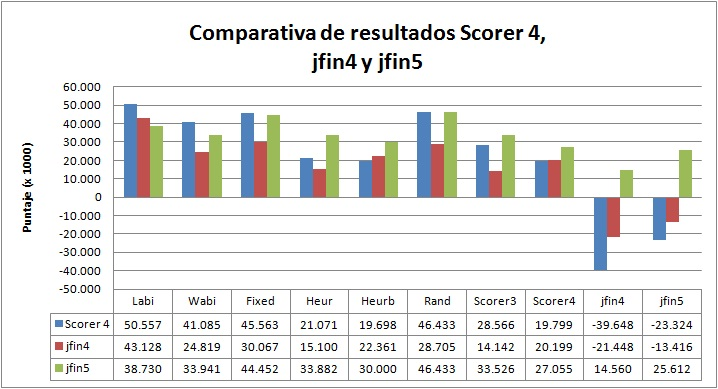
\includegraphics[scale=0.90]{graficos/3-1.jpg} \\
\scriptsize{\textsf{\textbf{Gr\'afico 3.1, comparación de los rendimientos obtenidos jugando con rojas de los tres jugadores importantes con sus parámetros ideales contra los jugadores de la cátedra y ellos mismos}}}  \\
\end{center}





\end{document}